\Chapter{Működés, tesztelés}

A fejezet az elkészített alkalmazás rendeltetésszerű működését mutatja be.

\Section{Config fájl}
Az alkalmazáshoz szükséges fájlok elérési útvonalát a config.xml fájlban kell megadni.
Egy fájl elérési útvonalát az alábbi módon kell megadni: \\C:\textbackslash Users\textbackslash AMD\textbackslash Desktop\textbackslash firebase\_service\_key\_example.json.
\vspace{5pt}\\Ha az alkalmazást először futattjuk az eszközön, vagy egy új mappában tettük a futtatható .jar fájlt, amiben nem található config.xml, akkor automatikusan létrejön az adott mappában egy fájl, példa adatokkal. Ezeket meg kell változtatnunk, hogy használni tudjuk az alkalmazást.
\vspace{15pt}\\A 6.1-es ábra egy automatikusan létrehozott config.xml fájl felépítését mutatja. A pirossal számozott sorok tartalmát kell szerkesszük, a további alfejezetekben ezt fejtem ki.
\begin{figure}[h]
	\centering
	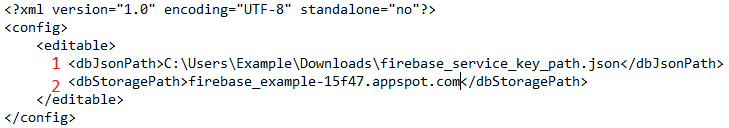
\includegraphics[scale=0.5]{images/config_1.png}
	\caption{Config.xml tartalma első futtatás után}
	\label{fig:config_file}
\end{figure}

\subsection{Firebase}
Az 1-es és 2-essel jelölt sorok megfelelő kitöltéséhez létre kell hoznunk egy Firebase adatbázist. 
\vspace{5pt}\\Egy böngészőben a \textit{console.firebase.google.com} url beírása, majd egy google fiókba való belépés után ez a 6.2 ábrán látható kép fogad minket.

\begin{figure}[h]
	\centering
	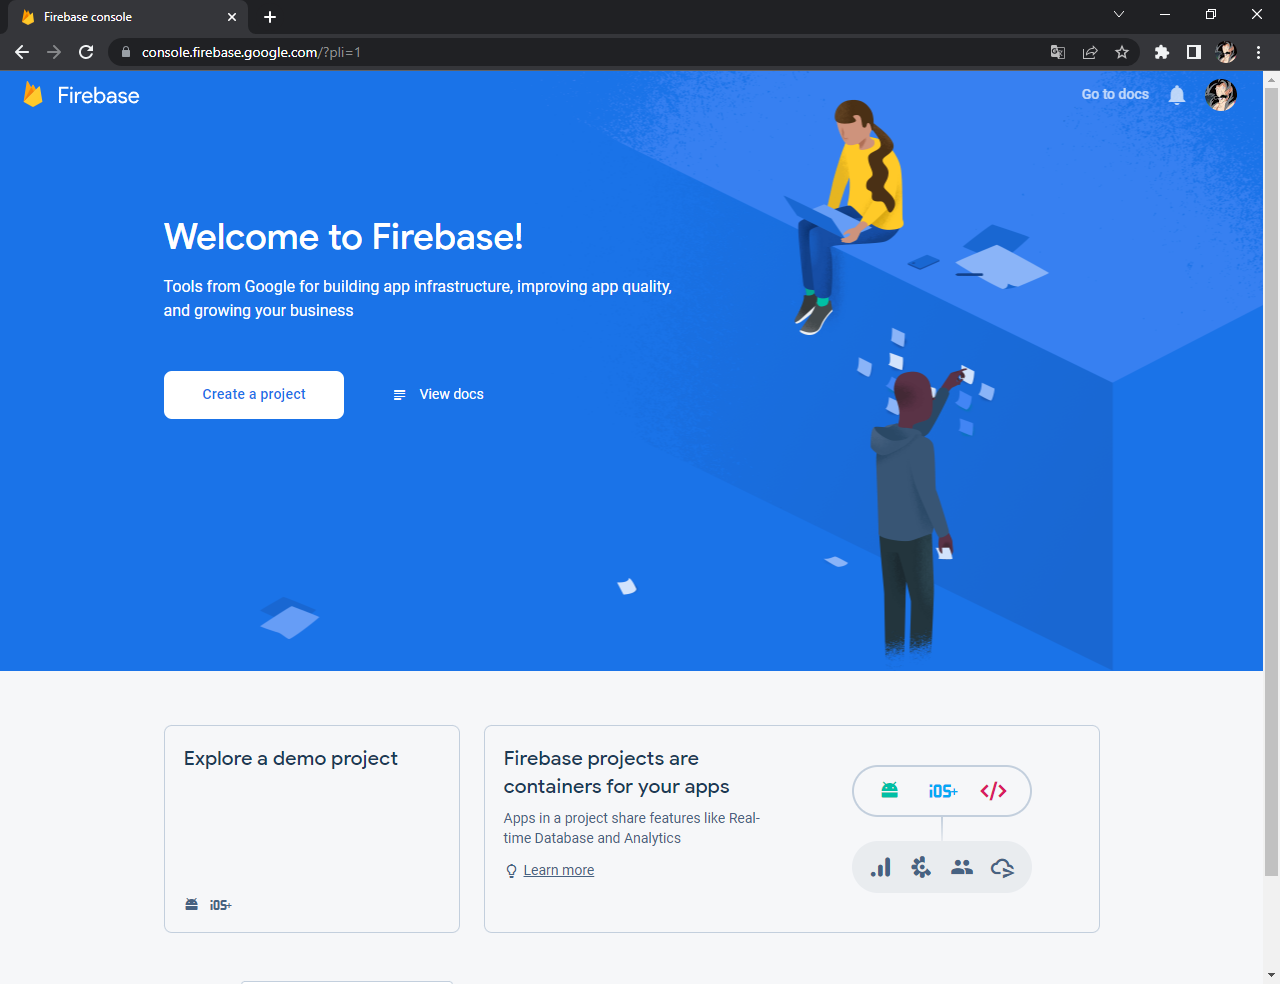
\includegraphics[scale=0.2]{images/config_2.png}
	\caption{Firebase regisztráció}
	\label{fig:firebase_reg}
\end{figure}
\noindent Kattintsunk a 'Create a project' gombra, majd végezzük el a szükséges lépéseket.
\\Ha megtettük, a 6.3 ábra képét láthatjuk. Kattintsunk a 'Storage' gombra a 'Build' menün belül a képernyő bal szélén található sávban.

\begin{figure}[h]
	\centering
	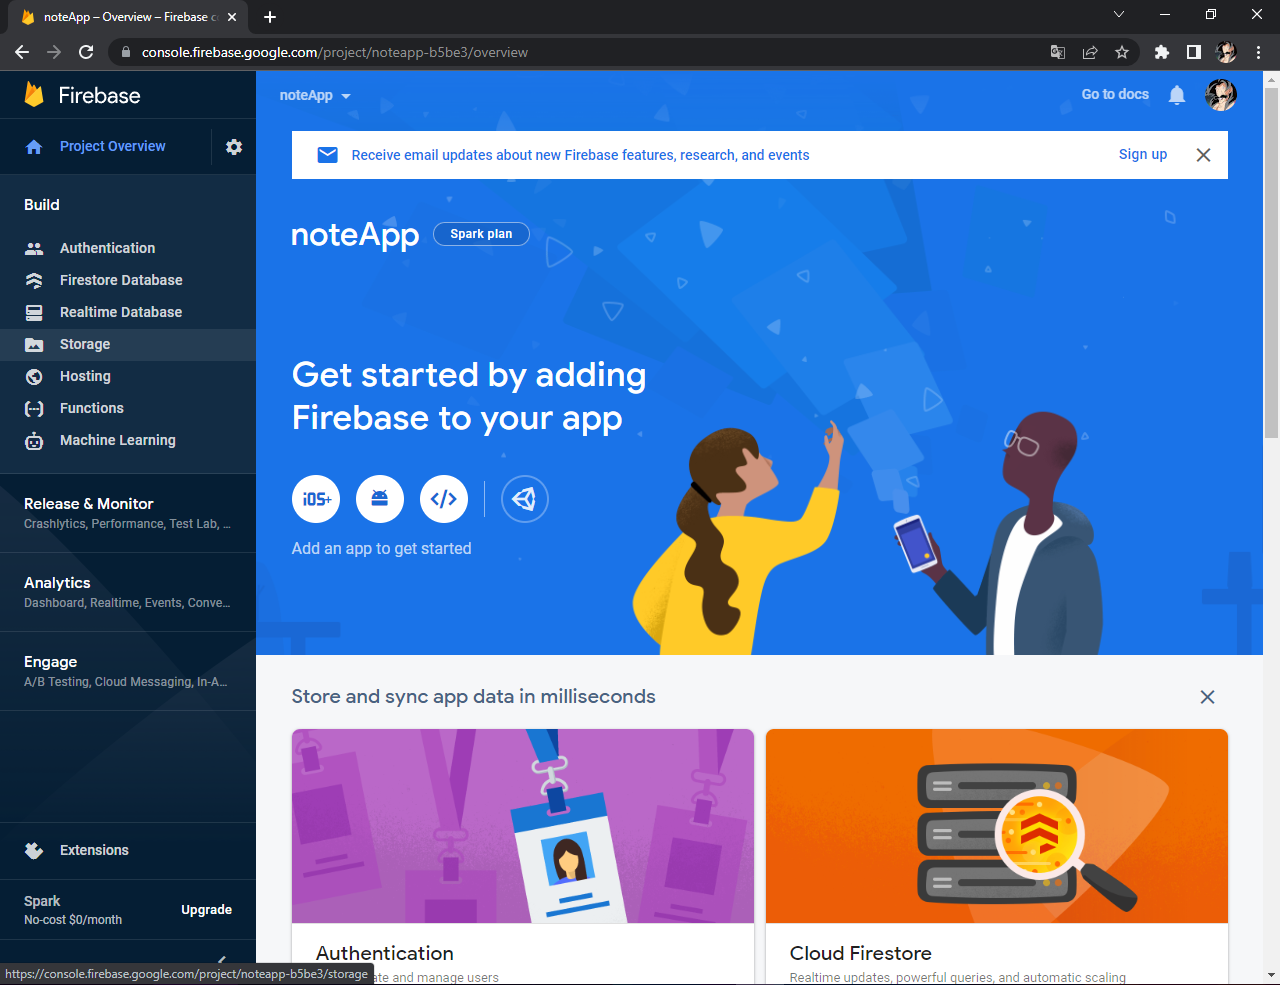
\includegraphics[scale=0.2]{images/config_3.png}
	\caption{Firebase kezdő képernyő}
	\label{fig:firebase_storage_reg}
\end{figure}

\noindent Kattintsunk a 'Get started' gombra, majd válasszuk ki a 'Start in production mode' lehetőséget, majd 'Next'. A legördülő menüben válasszuk a megfelelő Storage location-t, ami valószínűleg eur3 (europe-west) lesz. Fontos, hogy ezt nem lehet később megváltoztatni, így győződjünk meg választásunkról! Végül a 'Done' gombra nyomjunk.
\vspace{5pt}\\Ha ezt mind megtettük a 6.4-es ábrához hasonlót látunk.

\begin{figure}[h]
	\centering
	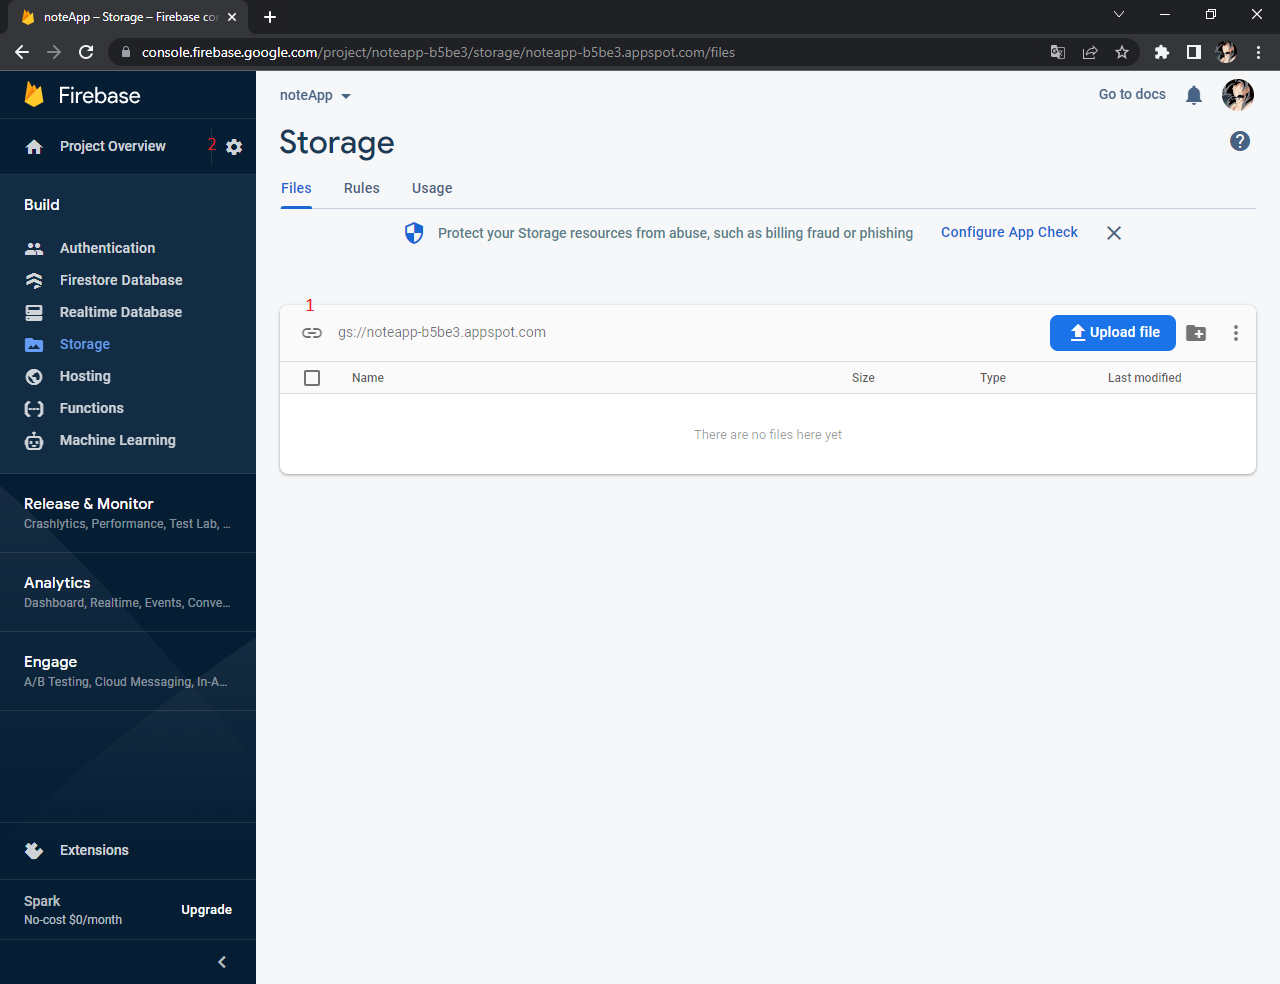
\includegraphics[scale=0.2]{images/config_4.png}
	\caption{Firebase storage alapértelmezett kép}
	\label{fig:firebase_storage_default}
\end{figure}







\noindent A config.xml fájlban a tag-ek (<dbJsonPath>...</dbJsonPath>) közé kell a megfelelő adatokat beírnunk. A 2-essel jelölt <dbStoragePath>...</dbStoragePath> tag-ek közé a 6.4-es ábrán 1-essel jelölt linket kell bemásoljuk a gs:// nélkül.
\vspace{5pt}\\Ha ez megvan kattintsunk a 6.4-es ábrán piros 2-essel jelölt fogaskerékre, majd 'Project settings', az újonnan megjelent felső sávban pedig a service accounts-ra (lásd 6.5 ábra 3-mas lehetőség).

\begin{figure}[h]
	\centering
	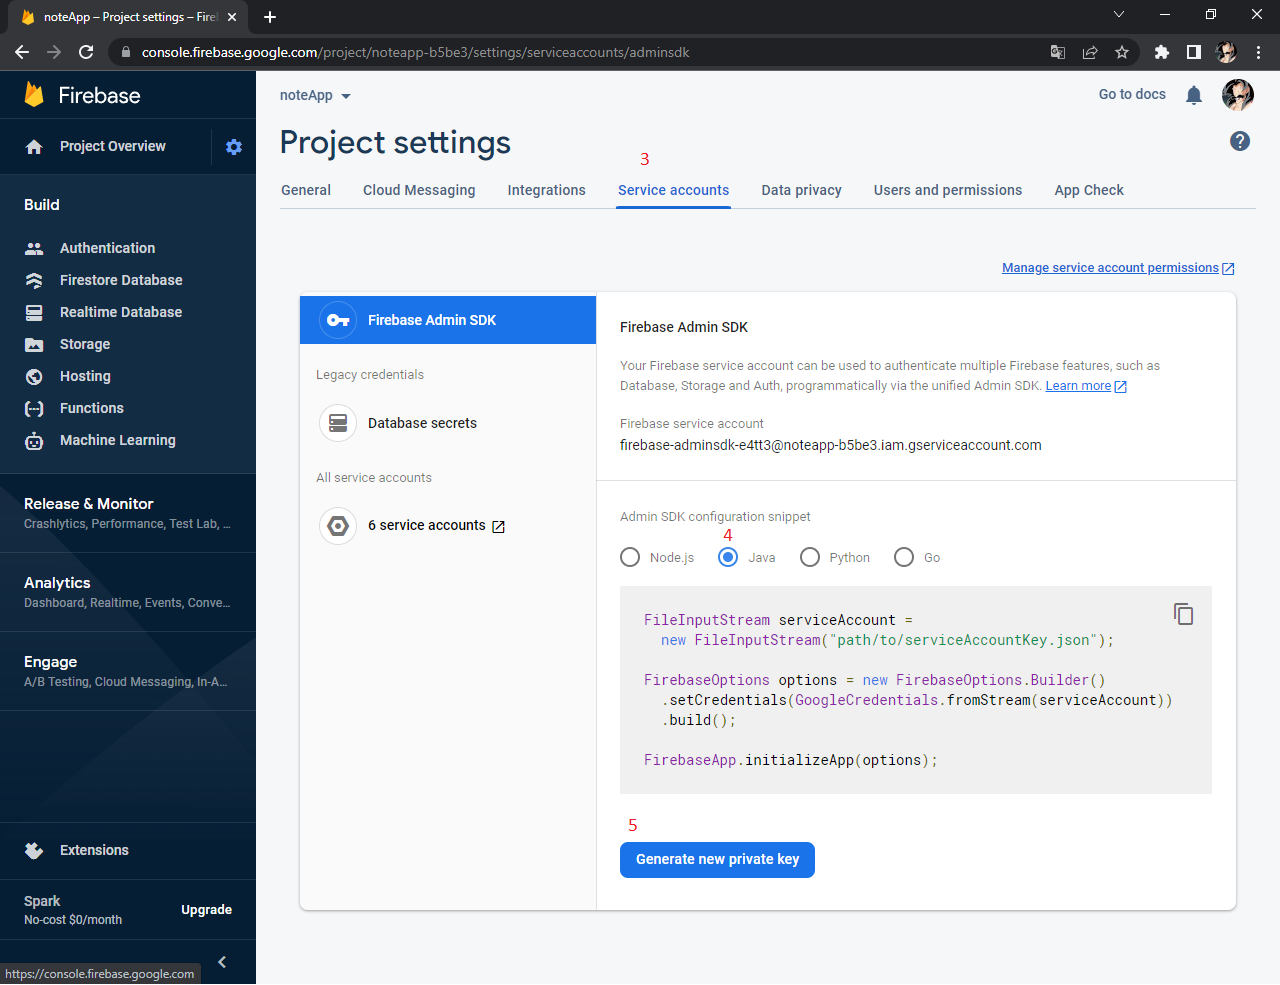
\includegraphics[scale=0.2]{images/config_5.png}
	\caption{Firebase service key generálás}
	\label{fig:firebase_service_key}
\end{figure}
\noindent Nyomjuk meg sorrendben a 6.5-ös ábrán piros számokkal jelölt gombokat, majd a felugró ablaknál a 'Generate key' gombot. Sikeresen letöltöttük a szükséges Firebase service key json fájlt!
\vspace{5pt}\\A config.xml fájlban a <dbJsonPath>...</dbJsonPath> tag-ek közé másoljuk be a letöltött json fájl elérési útvonalát. Ezt a leírás elején található példa elérési úthoz hasonlóan tegyük.
\vspace{5pt}\\ Ha lépésről lépésre mindent megtettünk, a config.xml fájl tartalma hasonlóan kell, hogy kinézzen, mint a 6.6-os ábrán látható.
\begin{figure}[h]
	\centering
	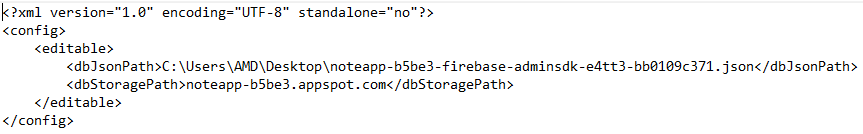
\includegraphics[scale=0.5]{images/config_6.png}
	\caption{Korrekt config.xml felépítés}
	\label{fig:config_file_final}
\end{figure}
\newline
\noindent Végezetül mentsük el, majd zárjuk be a config.xml fájlt, ezután futtassuk a .jar fájlt. Ha hibaüzenetet kapunk vizsgáljuk meg a config.xml fájlt. Nézzük meg, hogy helyesen írtuk-e be az elérési útvonalakat, '\textbackslash' jeleket alkalmaztunk-e a megadásukhoz. Ha továbbra is hibaüzenetet kapunk ismételjük el elejéről a lépéseket.
\vspace{5pt}\\ Ha mindent megfelelően adtunk meg a program elindul.


\subsection{Fontos információk}
\textbf{Nagyon fontos}, hogy a .jks fájlt ne töröljük. Ha mégis letöröljük hibákba fogunk ütközni, az alkalmazás adatai elvesznek és nem tudjuk őket sehogy visszaszerezni.
\vspace{5pt}\\Ha mégis törölnénk a KeyStore fájlt, akkor 6.4-es ábrán lévő felületen töröljük a Storage-ben lévő fájlokat. Így az előzőleg elmentett titkosított adatok is eltűnnek, és a .jks fájl is. A program ebben az esetben következő futtatáskor új fájlokat generál és üres tartalommal indul.


\newpage\Section{Jegyzetek menü}

Az 6.7-es ábrán látható a jegyzetek menü felépítése, a pirossal számozott elemek leírása található a kép alatt.

\begin{figure}[h]
	\centering
	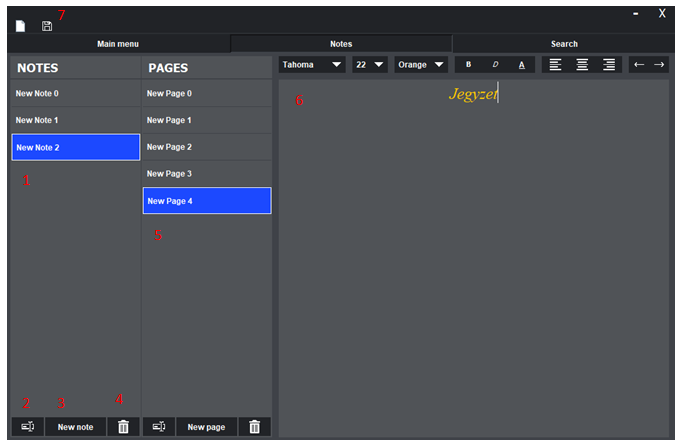
\includegraphics[scale=0.5]{images/doc_1.png}
	\caption{Jegyzetek menü használat közben.}
	\label{fig:menu_notes_2}
\end{figure}

\vspace{5pt} \noindent \textbf{1}-es panel a jegyzetek panelje, itt találhatóak egymás alá beszúrva a különböző jegyzetek. Az éppen kijelölt jegyzet kék színű, kattintással tudunk új jegyzetet kiválasztani, valamint ha a panelen belül az üres részre kattintunk, akkor mindig az utolsó jegyzetet fogja kijelölni.
\newline \\ Található a panelen 3 gomb. 
\vspace{5pt} \\ \textbf{2}-es gomb az éppen kijelölt jegyzet átnevezésére szolgál, egy felugró modális ablakba a beírt szövegre nevezhetjük át a kijelölt elemet, vagy megszakíthatjuk az egész folyamatot. (lásd 6.8 ábra)

\begin{figure}[h]
	\centering
	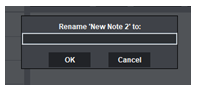
\includegraphics[scale=0.6]{images/doc_2.png}
	\caption{Átnevezésre szolgáló modális ablak.}
	\label{fig:menu_notes_rename}
\end{figure}

\vspace{5pt} \noindent \textbf{3}-mas gombbal új jegyzetet adunk a meglévő jegyzet listához. Alapértelmezett neve a jegyzeteknek ’New Note [sorszám]’. A sorszám a jegyzet id-jével egyezik, nem a listabeli pozíciójával.
\vspace{5pt} \\ \textbf{4}-es gombbal az éppen kijelölt jegyzetet törölhetjük, vagy szakíthatjuk meg ezt a folyamatot egy felugró modális ablak segítségével. (lásd 6.9 ábra)

\begin{figure}[h]
	\centering
	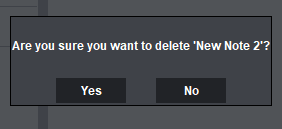
\includegraphics[scale=0.6]{images/doc_3.png}
	\caption{Törlésre szolgáló modális ablak.}
	\label{fig:menu_notes_delete}
\end{figure}

\vspace{5pt} \noindent \textbf{5}-ös panel a lapok panelje. Minden jegyzetnek külön lapjai lehetnek. A panel egyéb funkciói és kezelése teljesen megegyezik az előbb bemutatott jegyzetek menüével.
\vspace{5pt} \\ Ahogy kattintással váltogatunk a jegyzetek között, úgy frissül a lapok menü is, tehát ahogy a beszúrt képen látszik, az ’Egyetemi tárgyak’ jegyzetnek 4 lapja van. Ha átkattintanánk a ’TODO’-ra, akkor ebben a jegyzetben található lapok listája jelenne meg. Alapvetően jegyzet váltáskor nem jelölődik ki egy lap sem. 
\vspace{10pt} \\ \textbf{6}-os szövegdoboz felületen az éppen kijelölt lap tartalma jelenik meg. A felület mindig frissül, ha új lapra kattintunk, valamint ha nincs egy lap sem kijelölve, akkor üres lesz.
\\A szövegdoboz felett gombok találhatók, amik a szöveg szerkesztésére használhatóak.
\\Balról  jobbra haladva a gombok: 
\vspace{5pt} \\-Szöveg stílus váltás: alapértelmezett Tahoma. Csak a kijelölt szövegrész stílusa fog megváltozni!
\vspace{5pt} \\-Szöveg méret váltás: alapértelmezett 14-as méret. Csak a kijelölt szövegrész mérete fog megváltozni!
\vspace{5pt} \\-Szöveg szín váltás: alapértelmezett fehér szín. Csak a kijelölt szövegrész színe fog megváltozni!
\vspace{5pt} \\-Félkövér betű: kijelölt szövegrész félkövérré alakítása.
\\Gyorsbillentyű: Ctrl + B
\vspace{5pt} \\-Dőlt betű: kijelölt szövegrész dőltté változtatása.
\\Gyorsbillentyű: Ctrl + I
\vspace{5pt} \\-Aláhúzás: kijelölt szövegrész aláhúzása.
\\Gyorsbillentyű: Ctrl + U
\vspace{5pt} \\-Undo gomb: A szövegdoboz utolsó változtatását visszavonja. Fontos, hogy csak a szövegdobozon működik, note vagy page törlésre, átnevezésre, stb… nem!
\\Gyorsbillentyű: Ctrl + Z
\vspace{5pt} \\-Redo gomb: Az undo gomb ellentéte. Fontos, hogy csak a szövegdobozon működik, note vagy page törlésre, átnevezésre, stb… nem!
\\Gyorsbillentyű: Ctrl + Y

\vspace{5pt} \noindent \textbf{7}-essel jelzett gomb a mentés gomb. Gyorsbillentyű: Ctrl + S. Az alkalmazás tartalmát titkosítja majd elmenti az adatbázisba.
\\A gomb megnyomásakor vagy gyorsbillentyű használatakor az alkalmazás kis időre megfagyhat.




\newpage \Section{Kereső menü}

Az 6.10-es ábrán látható a kereső menü felépítése, a pirossal számozott elemek leírása található a kép alatt.

\begin{figure}[h]
	\centering
	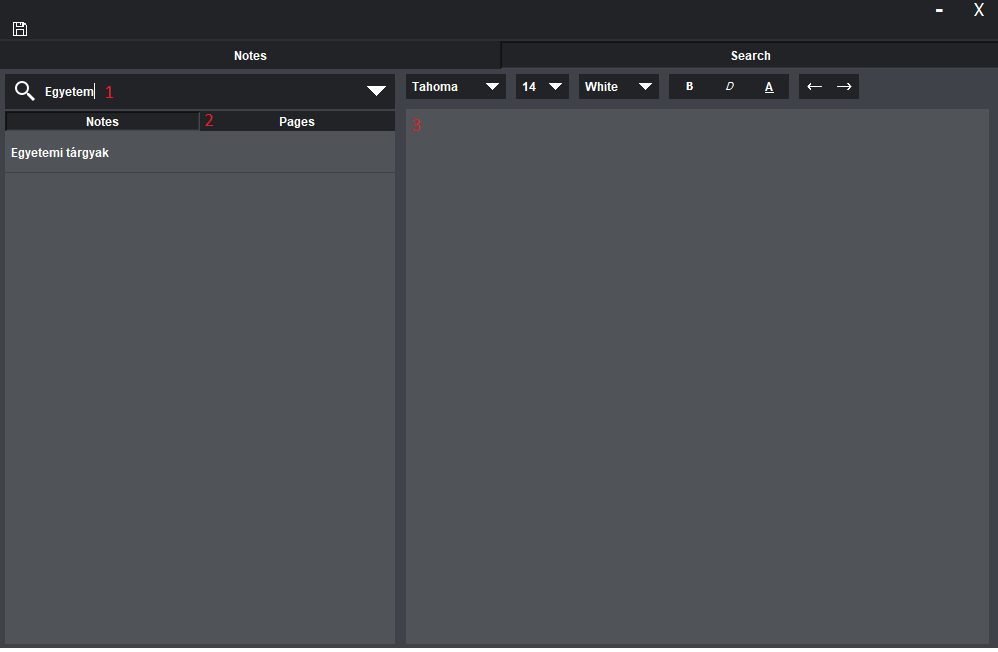
\includegraphics[scale=0.5]{images/doc_4.png}
	\caption{Kereső menü működés közben.}
	\label{fig:menu_search_2}
\end{figure}

\vspace{5pt} \noindent \textbf{1}-essel jelölt elem a ’search bar’ (kereső sor). Jegyzetek, lapok és lapok tartalma között keres. Ha jegyzet neve, lap neve, vagy lap tartalma tartalmazza a beírt kifejezést, akkor lesz találat. 
\vspace{5pt} \\Hogy a keresés könnyebb legyen, üres search bar-ba való kattintáskor az összes jegyzet és lap neve megjelenik egy listába. Ahogy a keresendő szöveget írjuk be a lista annak megfelelően fog változni. 

\begin{figure}[h]
	\centering
	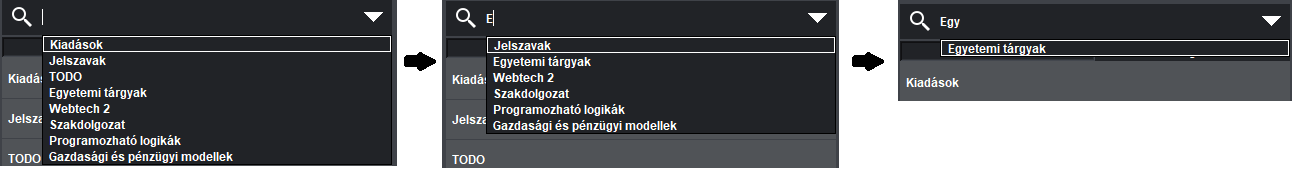
\includegraphics[scale=0.4]{images/doc_5.png}
	\caption{Keresési folyamat szemléltetése.}
	\label{fig:menu_search_searchBar}
\end{figure}
	
\vspace{5pt} \noindent Ha nincs egyezés, a lista eltűnik, nem jelenít meg egyetlen elemet sem.
\vspace{5pt} \\Ha az egyező szöveg egy adott lap tartalmán belül található, tehát nem a nevében, akkor is a listában a lap neve fog szerepelni.
\vspace{5pt} \\A beírt szövegre keresni kijelölés után a nagyítóra való kattintással vagy enter megnyomásával lehetséges.
	
	
\vspace{10pt} \noindent \textbf{2}-essel jelölt elem a Note és Page keresési találatok listája.
\vspace{5pt} \\Alapvetően, ha futtatáskor először lépünk be ebbe a menübe egyik sem lesz kijelölve, viszont az első keresés után a jegyzetek listáját fogja megjeleníteni. Hogyha a page-re kattintunk, akkor a talált lapokat fogja megjeleníteni, így tudunk váltani a talált jegyzetek és lapok, illetve lapok tartalma között.
\vspace{5pt} \\Ha a jegyzet találatok között az egyikre rákattintunk, akkor visszakerülünk a Notes Menu-be, hogy meg tudjuk tekinteni az adott jegyzet lapjait, átnevezni vagy törölni tudjunk.
\vspace{5pt} \\Ha a lap találatok között az egyikre kattintunk, akkor nem kerülünk vissza a Notes Menu-be. Az adott lap tartalmát tudjuk szerkeszteni és megtekinteni egy Notes Menu-höz hasonló szövegdobozban \textbf{(3.elem)}. Ennek funkciói teljesen megegyeznek az említett szövegdobozéval és menteni is a ctrl+s-el kell a változtatásokat, vagy a mentés ikonra kattintva.
\vspace{5pt} \\Ha esetleg átnevezni vagy törölni szeretnénk az adott lapot, a Notes Menu-ben tehetjük ezt meg.

\Section{Ismert bug-ok}
Jelenleg két kisebb bug-ról tudok, ami biztosan megtalálható az alkalmazásban. Egyik bug sem 'töri meg' az alkalmazást, de a gördülékeny működéshez jó lenne a közeljövőben megoldani őket.
\\ Mind a felhasználói felülethez köthető, azon belül is a kereső menühöz.
\begin{itemize}
	\item Bármit írunk be a keresőbe, ha több mint egy találatot dob ki, és rányomunk az első lehetőségre, akkor az a keresősáv szövegdobozába mindig a 'New Note 0'-t fogja behelyettesíteni (a jegyzetek listájának első elemének nevét). Ez egyetlen egyező találat esetén nem érvényes.
	\item A másik keresősáv bug pedig ehhez, egyetlen egyezés esetéhez köthető. Tegyük fel rákeresünk a 'New Note 0'-ra, akkor a legördülő menü eltűnik, attól függetlenül, hogy van egyező találat. A szövegdobozra való újabb kattintással jelenik meg. Ha viszont nem teljes egyezőséggel keresünk rá valamire, például azt írjuk be, hogy 'New note 0', akkor megjelenik az egyező találat egyetlen egyezés esetén is. Valamilyen case-sensitive probléma lehet, amire sajnos nem tudtam rájönni.
	
\end{itemize}
\noindent Szóba kerültek az 5.5 és 5.6 alfejezetben a felhasználói felület létrehozásával kapcsolatos nehézségek, a felsorolt bug-okat is ilyen nehézségnek tudnám be. 
\\Úgy gondolom, ha nem Swing-et, hanem egy modernebb GUI fejlesztő függvény könyvtárat használtam volna, akkor nem találkoztam volna ezekkel a hibákkal.